\documentclass[12pt,a4paper,twocolumn]{article}

% --- Page layout / typography (per brief) ---
\usepackage[a4paper,margin=2.5cm]{geometry}
\usepackage{setspace}
\setstretch{1.0} % single spacing
\usepackage[T1]{fontenc}
\usepackage[utf8]{inputenc}
\usepackage{lmodern}
\usepackage{microtype}

% --- Figures / tables ---
\usepackage{graphicx}
\usepackage{booktabs}
\usepackage{array}
\usepackage{tabularx}
\usepackage{multirow}

% --- Lists / links ---
\usepackage{enumitem}
\setlist{nosep}
\usepackage[hidelinks]{hyperref}

\usepackage{amsmath}
% --- References ---
\usepackage[numbers]{natbib}

% --- Optional: reduce whitespace around headings ---
\usepackage{titlesec}
\titlespacing*{\section}{0pt}{0.9\baselineskip}{0.4\baselineskip}
\titlespacing*{\subsection}{0pt}{0.7\baselineskip}{0.3\baselineskip}

\usepackage{titling}
\setlength{\droptitle}{-2cm}  % adjust: -0.8cm to -1.5cm typical
% --- Small helpers ---
\newcommand{\todo}[1]{\textbf{[TODO: #1]}}

\setlength{\textfloatsep}{8pt plus 2pt minus 2pt}
\setlength{\floatsep}{6pt plus 2pt minus 2pt}
\setlength{\intextsep}{6pt plus 2pt minus 2pt}

\title{Technical Milestone Report: Automatic Synthesis of Virtual Model Controllers for Robotic Manipulation}
\author{Hasan Shahrestani (smhs4)}

\begin{document}

\maketitle

\begin{abstract}
\textbf{Summary.} This project investigates whether \,\emph{Virtual Model Controllers (VMCs)}\, for manipulation can be generated automatically rather than designed by hand. The current approach uses a genetic algorithm (GA) to search over both (i) the \emph{structure} of a VMC represented as a network of virtual springs/dampers (tendons) between robot and object sites, and (ii) the continuous parameters (stiffness, damping, rest length). Progress to date includes: a working end-to-end GA training pipeline in MuJoCo; multiple iterations of the fitness function; improved genome encoding and genetic operators; parallel evaluation; and initial tests on pickup and mesh-based objects.
\end{abstract}

\section{Motivation and project objectives}
Robot manipulation remains difficult to engineer reliably because contact-rich interaction, friction variability, and object diversity make controller design highly task-specific \cite{suomalainen2021contactsurvey}. Virtual Model Control offers an intuitive way to produce compliant motion by attaching \emph{virtual} springs, dampers and masses to the robot and object, generating torques that mimic physical interaction \cite{pratt2001vmc}. However, hand-crafted VMCs are time-consuming to tune, custom-made per task, and do not scale well to more complicated behaviours.

\subsection{Overall aim}
The aim of this project is to automatically synthesise a VMC from a manipulation task definition (e.g., \emph{pick up the object}) by searching for:
\begin{itemize}
    \item A virtual component \textbf{structure}: which parts of the robot and objects are connected to each other via springs and dampers.
    \item Continuous \textbf{parameters}: spring stiffness, damping and rest length.
\end{itemize}

\subsection{Success criteria (milestone-level)}
By the end of the project, success will be measured by:
\begin{itemize}
    \item Demonstrating consistent `task completion' in simulation across varied initial object poses (robustness).
    \item Producing controllers that transfer to at least one real-robot manipulation test with safety constraints. (sim to real)
    \item Providing a clear methodology: encoding, fitness design, and optimisation settings that can be reused and applied to other robot manipulation tasks.
\end{itemize}

\section{Methodology}
% \subsection{System overview and long-term vision}

% In this project, the \textit{Sciurus 17-DoF humanoid robot} is selected as the target manipulation platform. This robot is particularly well suited to the proposed research due to its dual-arm configuration, which enables the study of coordinated bimanual manipulation and richer interaction strategies than single-arm systems.

% The overarching vision of the project is to develop an end-to-end manipulation pipeline in which
% \begin{enumerate}
%     \item the robot first perceives a target object using visual sensing, such as RGB cameras or 3D point clouds and categorises it.
%     \item Based on this categorisation and the target task, an appropriate control policy is selected and deployed. This policy is represented as a Virtual Model Control (VMC) mechanism.
%     \item In a real-world deployment, the VMC parameters can be finetuned for the specifics of the current situation using model predictive control by simulation.
%     \item The robot would ultimately act under this VMC-based controller to complete the desired manipulation task for a wide range of target behaviours and object characteristics.
% \end{enumerate}

% While this full perception-to-action pipeline represents the final vision of the project, its complete implementation is beyond the scope of the current milestone.

% Instead, the initial focus of this work is deliberately constrained to a well-defined and tractable subproblem. Specifically, the project aims to generate an effective VMC for a particular object geometry with known range for mass and size, where the simulated and real-world instances are identical or only slightly different. Genetic Algorithms (GA) are used to optimise the VMC parameters entirely within simulation. Once a satisfactory controller is obtained, it is transferred to the real robot and evaluated without further learning.

% In practice, this approach implies that for each distinct object shape and target manipulation behaviour, a separate GA optimisation must be performed. This assumption simplifies the problem at this stage and provides a clear foundation for future work, where generalisation across object classes and tasks could be explored. Ofcourse vision is still required in this case for object tracking since the virtual components need to track the position and velocity of the object they are attached to.


\subsection{VMC Synthesis Pipeline}
\subsubsection{Simulation setup}
Experiments are carried out in MuJoCo using an upper-body humanoid platform (Sciurus17) and a simplified grasping setup. The current testbed uses simplified end-effectors (``chopsticks'' or planar grippers) and a small object to evaluate grasp and lift behaviours. The same pipeline is being extended to mesh-based objects. \\
\textbf{Extension:} 
\begin{itemize}
    \item Incorporate \textbf{soft or compliant materials} in simulation to improve gripping performance and better reflect real-world contact interactions.
    \item Enable \textbf{greater object diversity} during training by supporting deformable or semi-compliant objects, increasing robustness and generalisation.
    \item Explore \textbf{simulation speed optimisations}, by adjusting parametrs to balance between realism and efficiency or exploring computional hacks such as using a GPU to increase speed.
\end{itemize}


\subsubsection{VMC search space}
A VMC candidate is represented as a set of tendons (virtual springs/dampers) between predefined \emph{sites} (Fig.~\ref{fig:robot})  on/relative-to the robot and the object. Each tendon is parameterised by:
\begin{itemize}
    \item stiffness $k$ and damping $c$ (continuous),
    \item rest length $\ell_0$ (continuous, optionally enabled),
    \item endpoints: indices of robot/object sites (discrete).
    \item number of spring and dampers in the controller
\end{itemize}
\textbf{Extension:} The search space is currently limited:
\begin{itemize}
    \item Number of possible spring and dampers are fixed
    \item sites are predefined discrete points.
    \item Constant. Once set parameters do not change during operation. Parameters espcially continues ones should be time varying.
\end{itemize}
Finding efficient ways of searching the space while ensuring stability will allow these limitations to be reduced.

\subsubsection{Optimisation algorithm}
A genetic algorithm (GA) evolves a population of candidate controllers by repeated evaluation, selection, crossover and mutation \cite{man1996ga}. Key GA hyperparameters include
\begin{itemize}
    \item population size, number of generations, tournament size, crossover/mutation probability and elitism.
    \item \textbf{encoding} which defines how each candidate VMC mechanism is represented, and dictates how they are crossed-over/mutated.
    \item \textbf{crossover/mutation mechanisms} which govern how encodings are manipulated and combined.
\end{itemize}
\textbf{Extension:}
While the GA has demonstrated reliable convergence to effective VMC designs at reasonable computational cost, several extensions and alternative optimisation strategies may be explored.

\begin{itemize}
    \item \textbf{Neural network--based controllers and Reinforcement learning approaches}, RL algorithms which are designed for fixed horizon, final reward scenarios sush as GRPO \cite{yuan2024grpo} seems well suited for this task.
    \item \textbf{Hybrid methods}, combining GA-based structural optimisation with learning-based parameter refinement, could leverage the strengths of both global search and local optimisation.
\end{itemize}

% \item \textbf{Multi-objective optimisation} (e.g.\ stability, energy efficiency, robustness) may further improve controller performance and reduce overfitting to specific tasks.

% Recent iterations use simulated binary crossover (SBX) for continuous parameters  and explore .

\subsubsection{Fitness function}
Each task requires a fitness function to optimise so that quality of the proposed VMC can be quantified. In object manipulation \cite{sahbani2012grasp} this is a multi-objective function and depends on the task itself.
For example pickup task fitness currently combines task-specific signals such as \textbf{final object height} but general quality objective still remain: stability, efficiency, contact and robustness are all neccasary for a high grasp.
    
\textbf{Extensions:} The current fitness function combines multiple criteria using a linearly weighted sum with manually tuned weights. While effective, this approach can be improved in several ways:

\begin{itemize}
    \item \textbf{Objective normalisation}: scale individual fitness terms to comparable ranges to reduce sensitivity to arbitrary weighting and improve optimisation stability.
    \item \textbf{Multi-objective optimisation}: explicitly search for Pareto-optimal solutions (e.g.multi-objective GA concepts (e.g., NSGA-II) \citep{deb2002nsga2}) rather than collapsing all objectives into a single scalar fitness.
    \item \textbf{Structural constraints}: restrict the search space a priori by enforcing stability- and efficiency-aware design rules, reducing reliance on fitness penalties for infeasible or pathological solutions.
\end{itemize}

\subsection{Practical Implementation}
\begin{itemize}
    \item \textbf{Object tracking and perception:}
    The robot must estimate the object’s position, orientation, and (approximate) geometry to correctly instantiate the VMC and compute interaction forces.
    The Sciurus17 platform provides a 3D point-cloud camera that may be used to reconstruct object geometry and localise contact points.
    Alternative sensing solutions include classical computer vision pipelines or external motion-capture systems (e.g.\ OptiTrack) for higher accuracy.

    \item \textbf{Mapping MuJoCo tendons to robot torques:}
    The current MuJoCo model relies on built-in tendon abstractions applied to a gravity-compensated robot.
    On real hardware, equivalent behaviour must be achieved by converting virtual tendon forces into joint torques via an inverse Jacobian.
    Implementing this mapping explicitly in simulation would reduce the sim-to-real gap and better reflect the physical control pipeline. This is also required to match the torque limits of the robot. Currently induced torque is not calculated and therefore simulation results may not match reality.

    \item \textbf{Encoding translation and deployment:}
    A software tool is required to automatically convert the optimised GA encoding into a Julia-compatible VMC representation that can be executed on the robot.
    At present, this translation is performed manually and represents a clear opportunity for automation and improved reproducibility.

    \item \textbf{Real-world fine-tuning:}
    While large-scale GA optimisation is impractical on hardware due to sample inefficiency, limited real-world refinement may be performed after simulation training.
    This could include parameter fine-tuning or local adaptation to unmodelled dynamics, improving robustness without prohibitive data collection.

    % \item \textbf{High-level task coordination:}
    % A more general solution would incorporate an overarching controller responsible for switching between different VMC mechanisms.
    % This enables sequencing of behaviours to solve multi-step tasks (e.g.\ approach, grasp, lift, place), or adapting the active VMC based on task phase, object state, or sensory feedback.
    % Such a hierarchical structure separates low-level compliant interaction from high-level decision-making, improving modularity and reuse.
\end{itemize}

\section{Progress to date}
Significant progress has been made across four key milestones:
\begin{itemize}
    \item \textbf{Pipeline Development:} Established an end-to-end GA pipeline in MuJoCo. This includes parallel fitness evaluation, automated site/tendon generation, and support for mesh-based geometries (Fig.~\ref{fig:triangle}).
    \item \textbf{Genome Redesign:} Transitioned to a fixed-size matrix encoding (Fig.~\ref{fig:vmc-encoding}). By limiting the number of virtual components, we reduced search space growth and improved the effectiveness of genetic operators.
    \item \textbf{Algorithmic Refinement:} Implemented Simulated Binary Crossover (SBX) for continuous parameters and discrete crossover for topology. Robustness was enhanced by evaluating candidates across randomized initial object poses.
    \item \textbf{Preliminary Results:} Achieved consistent lifting for primitive blocks and pyramids. Results are also quantitatively assesed by viewing fitness function, improvements and maintaining popultion diversity (Fig.~\ref{fig:evolution_stats}). Current work is focused on refining contact stability for complex meshes.
\end{itemize}

% -------------------------------------
% \subsection{Milestone 1: Working GA pipeline and parameter exploration}
% A rudimentary end-to-end GA pipeline was implemented and tested under multiple parameter settings. Results were quatitavly (Fig.~\ref{fig:evolution_stats}) and visually assesed by seeing full simulation of the resulting VMC. As mentioned in Methodology section, the optimisation was very sensitive to fitness function weightings, GA encoding and GA parameters.

% \subsection{Milestone 2: Tooling and simulation improvements}
% Several engineering changes were made to support faster iteration:
% \begin{itemize}
%     \item Helper classes were created to allow automatic generation of sites, tendons, objects. 
%     \item Improved tooling to track and compare configuration changes across runs.
%     \item Parallel fitness evaluation across CPU cores to increase throughput.
%     \item Refinements to object and gripper geometry (increased contact area) and friction-related tuning.
%     \item Handling of unstable configurations by filtering/penalising invalid episodes.
% \end{itemize}
% Attempts were made to introduce soft-body objects in MuJoCo (flexcomp), but this did not perform reliably within the current time budget.

% \subsection{Milestone 3: Encoding redesign and improved genetic operators}
% The genome encoding was revised to something like Fig.~\ref{fig:vmc-encoding} As can be seen from the example this limits the number of total virtual components to 7, as mentioned before this reduces the search space growth and improves genetic operator effectiveness. The genetic operators were also updated:
% \begin{itemize}
%     \item SBX crossover for continuous parameters (stiffness, damping, length). \citep{deb1995sbx}
%     \item Discrete crossover (two-point) over tendon endpoint connections.
%     \item Mutation operators that perturb site indices and apply polynomial mutation to continuous parameters.
%     \item Fitness evaluated across multiple starting positions to reduce overfitting to a single initial state.
% \end{itemize}
% These changes produced more consistent pickup behaviours and enabled preliminary ``block rising'' and pickup successes; block flipping remains in progress.


% \subsection{Milestone 4: Extension towards mesh objects and faster compute}
% The codebase was extended with compatibility for mesh objects (Fig.~\ref{fig:triangle}) and tested on a pyramid-like object which yielded more successful results. Training is now also run on a server to increase compute throughput.

\subsection{Lessons learned}
\begin{itemize}
    \item \textbf{Search space / instability:} increasing tendon count and permissive encodings can produce unstable, unphysical behaviours.
    \item \textbf{Fitness shaping:} small changes to weighting can dominate selection and push the GA toward degenerate solutions (e.g., ``gaming'' centre/height terms).
    \item \textbf{Generalisation:} optimisation on a single initial pose can lead to brittle controllers; evaluating across multiple initial conditions improves robustness but increases compute cost.
    \item \textbf{GA parameter tuning:} Population size and generation number is an important factor in performance but comes at a computational cost. Mutation and cross over probability also need to be tuned to the size of the genome.
\end{itemize}

\section{Plan for remaining work}

The remainder of the project is prioritised around achieving a \emph{minimum viable sim-to-real transfer} for a single representative object and task, before expanding to robust and generalisable performance. VMC synthesis for simple task and general mesh objects are ready; therefore the critical path is implementing the practical deployment steps required for execution on the Sciurus17 robot, validating equivalence between simulation and hardware, and establishing safe repeatable trials.

\subsection{WP1: Minimum viable sim-to-real transfer (highest priority)}
\textbf{Goal:} execute a GA-trained VMC on the real robot for one target object and manipulation task, under safety constraints, with behaviour consistent with simulation. The steps for this are mentioned section 2.2 Practical Implementation. \\
\textbf{Timeline} - Weeks 1 \& 2 Lent

\begin{itemize}
    \item \textbf{Object tracking and state estimation.} Implement the minimum sensing pipeline required to estimate object pose (and optionally velocity) robustly enough to instantiate VMC sites.
    \item \textbf{Explicit VMC-to-torque mapping.} Replace any MuJoCo-specific abstractions with an explicit mapping from virtual component forces to joint torques via robot Jacobians.
    \item \textbf{Genome-to-deployment automation.} Build a reproducible conversion from the GA genome to a deployable VMC configuration (Julia-compatible controller representation), eliminating manual transcription.
    \item \textbf{Safety envelopes and staged deployment.} Define conservative torque/velocity limits and termination conditions.
\end{itemize}

\subsection{WP2: Fine-tuning and generalisation after first real success}
\textbf{Goal:} improve reliability and reduce sensitivity to modelling errors, and object initial pose and size after the first working sim-to-real demonstration. \\
\textbf{Timeline} - Week 3 \& 4 Lent

\begin{itemize}
    \item \textbf{Generalisation to more tasks and shapes:} Test on more complicated shapes and more sophisticated tasks.
    \item \textbf{Hardware calibration loop.} Identify which parameters cause the largest sim-to-real discrepancy (friction, compliance, controller gains, latency) and calibrate them using short diagnostic experiments.
    \item \textbf{Lightweight real-world refinement.} Introduce limited on-hardware tuning that is sample-efficient (e.g.\ local parameter search around the GA solution, or constrained updates), while keeping the bulk optimisation in simulation.
    \item \textbf{Robustness training in simulation.} Increase robustness by evaluating candidate controllers across distributions of initial poses and physical parameters (mass, friction), and enforce constraints aligned with the hardware safety limits.
\end{itemize}

\subsection{WP3: Improved optimisation and adaptive control (stretch goals)}
\textbf{Goal:} move beyond ``set-and-go'' controllers and object-specific optimisation towards controllers that generalise and adapt. \\
\textbf{Timeline} - Week 5 - 8 Lent
\begin{itemize}
    \item \textbf{Alternative optimisation algorithms.} Investigate whether a policy-gradient method (e.g.\ GRPO) can outperform GA in data efficiency or robustness once a stable torque-mapped simulation pipeline is available.
    \item \textbf{Time-varying VMC parameters.} Extend the representation so that stiffness/damping/rest length vary over time or by task phase (e.g.\ approach vs.\ grasp vs.\ lift), rather than remaining constant throughout an episode.
    \item \textbf{Multi-step / hierarchical control.} Introduce a higher-level mechanism to switch between multiple VMC primitives or parameter schedules to execute multi-stage tasks.
\end{itemize}


\section{Risk assessment}

\noindent\textbf{R1 (L: High, I: High) Sim to Real Gap}
Difficulty in accuratly tracking objects pose and shape, robot torque limits, inacurate contact simulations could all pose a signicant challenge.
\emph{Mitigation:} There are multiple options for object tracking that can be tested (optitrack, pointcloud). Also we will start with basic shapes with simple geometries. Iteration will allow us to tune simulation parameters to match reality more closely. This will all increase the required time but time pressure is not too high based on the current plan.

\noindent\textbf{R2 (L: Low--Med, I: High) Safety during trials.}
Optimised parameters may generate unsafe forces which can damage the robot and the object.
\emph{Mitigation:} hard caps and termination conditions, conservative bounds, contact-only trials before lift.

\noindent\textbf{R3 (L: Med, I: Med) Compute limits for generalisation}
Robustness training via GA may be too expensive.
\emph{Mitigation:} staged domain randomisation, parallel evaluation, prioritise pose/friction/mass. If none work, can switch to a more genralisable search algorithm.

\noindent\textbf{R4 (L: Med, I: Med) Advanced methods not ready.}
Alternative optimisers may not converge in time or may not work at all.
\emph{Mitigation:} keep as stretch goal; benchmark fairly against GA using identical evaluation.


\bibliographystyle{unsrtnat}
\bibliography{references}

\section{Appendix}
% --- Figure placeholders (optional) ---
\begin{figure}[h]
\centering
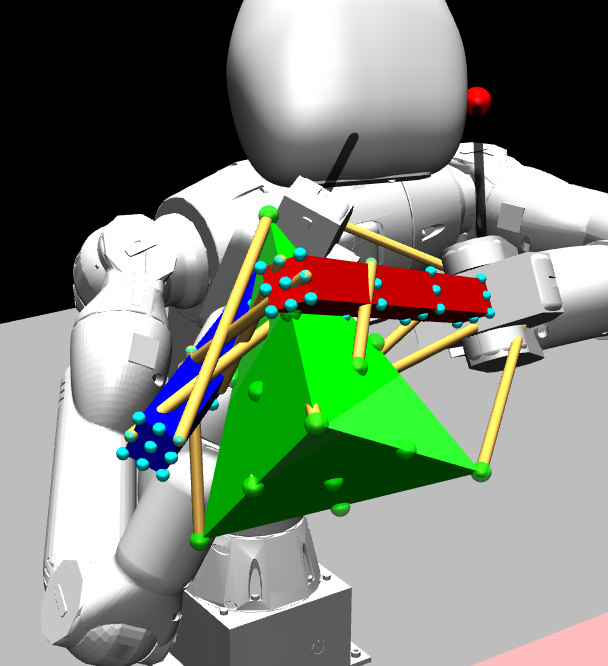
\includegraphics[width=0.6\linewidth]{figures/triangle_updated.png}
\caption{Optimisation pipeline supports mesh objects such as pyramid. sites are automatically added based on faces and edges}
\label{fig:triangle}
\end{figure}

\begin{figure}[h]
\centering
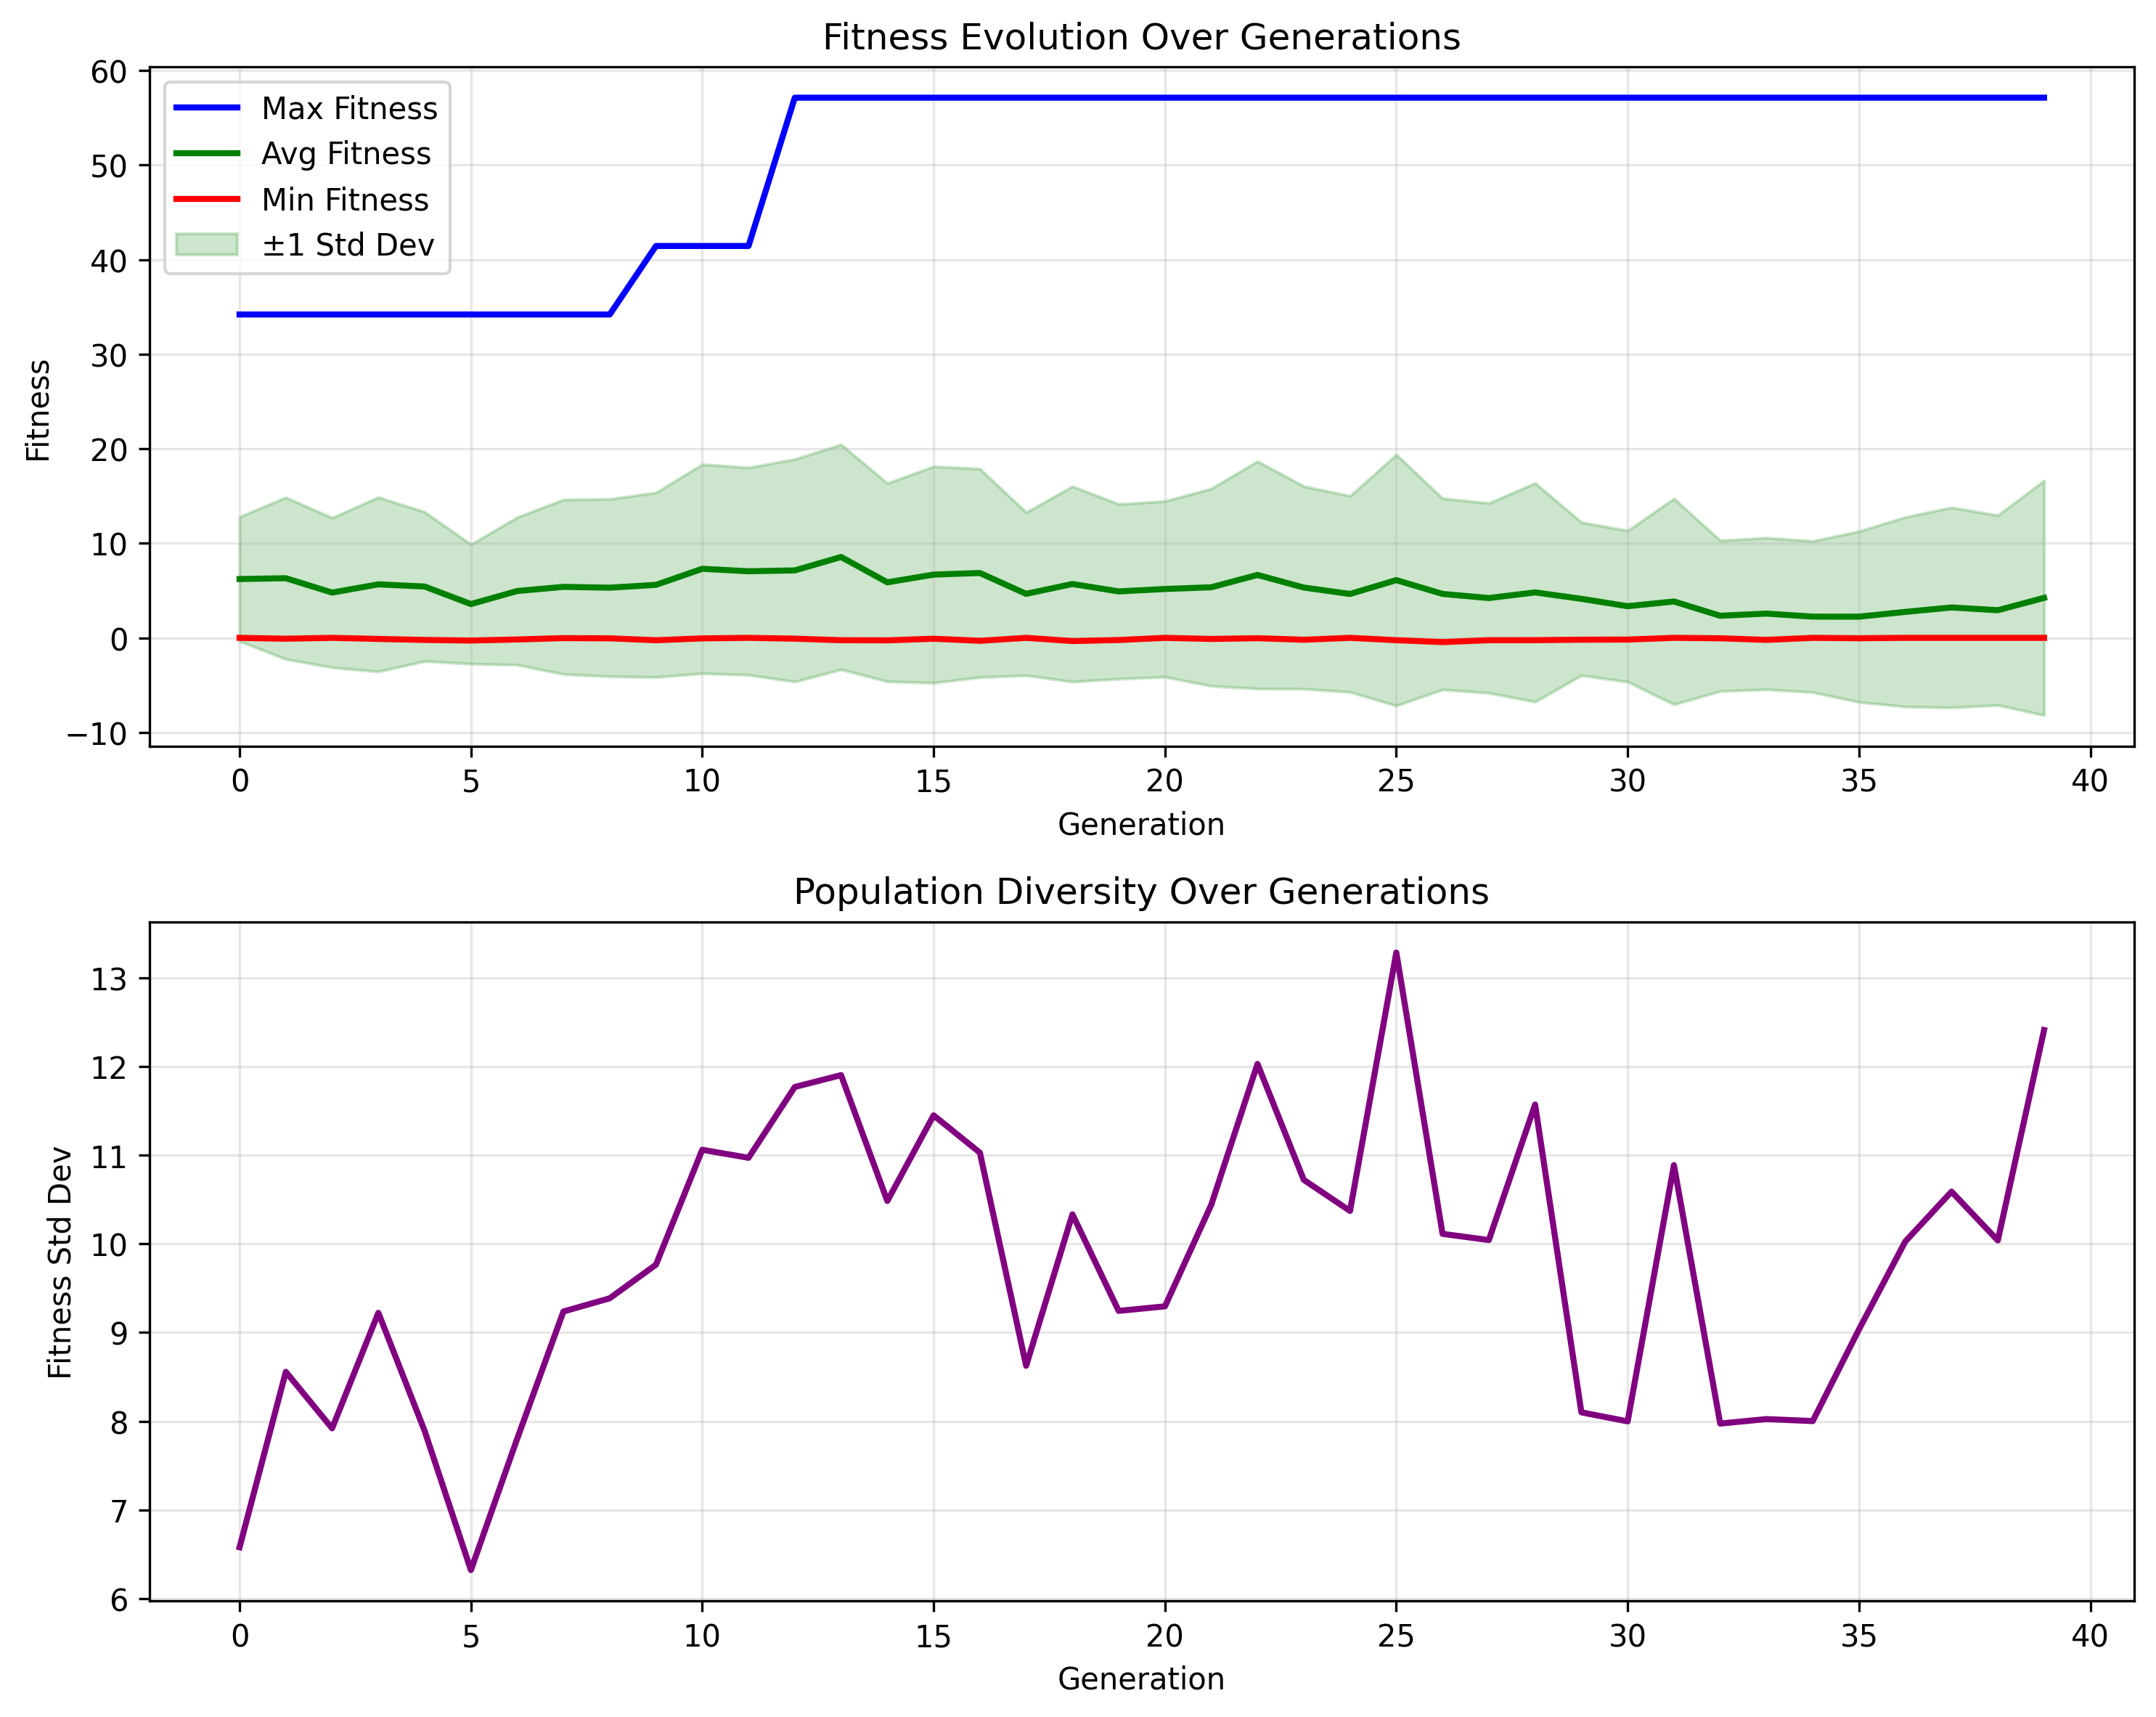
\includegraphics[width=0.6\linewidth]{figures/evolution_statistics.png}
\caption{Example evolution statics for a run of the GA algorithm.}
\label{fig:evolution_stats}
\end{figure}

\begin{figure}[h]
\centering
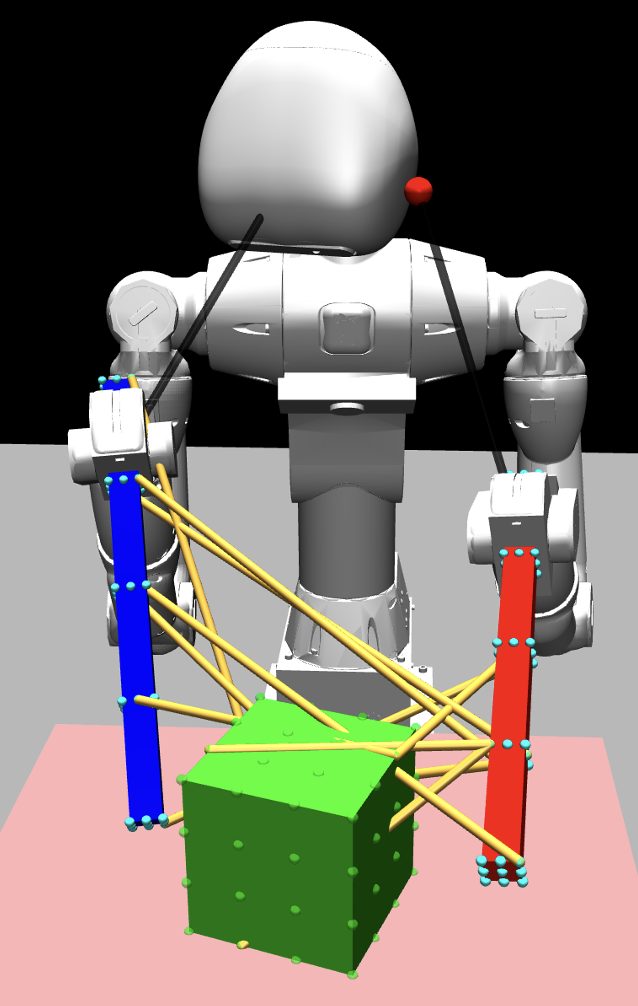
\includegraphics[width=0.6\linewidth]{figures/robot_sites_tendons.png}
\caption{Sciurus17 robot with replaced arms in MuJoCo simulation environment. Green and blue points are sites define on the arms and object. Yellow tendons are connected between sites based on GA encoding}
\label{fig:robot}
\end{figure}



\begin{figure}[h]
\centering
\[
\begin{array}{c}
\text{right to left} \\
\left(
\begin{array}{ccccc}
\text{SL1} & \text{SO1} & s & d & l \\
\text{SL2} & \text{SO2} & s & d & l \\
\text{SL3} & \text{SO3} & s & d & l
\end{array}
\right)
\\[6pt]
\text{left to object} \\
\left(
\begin{array}{ccccc}
\text{SR1} & \text{SO1} & s & d & l \\
\text{SR2} & \text{SO2} & s & d & l
\end{array}
\right)
\\[6pt]
\text{right to object} \\
\left(
\begin{array}{ccccc}
\text{SL1} & \text{SR1} & s & d & l \\
\text{SL2} & \text{SR2} & s & d & l
\end{array}
\right)
\end{array}
\]
\caption{Genome encoding for the virtual model controller. Each row represents a virtual spring--damper element defined by its endpoint sites and continuous parameters (stiffness $s$, damping $d$, rest length $l$).}
\label{fig:vmc-encoding}
\end{figure}



\end{document}
